\newpage
\section{Lectures and Tutorials}
\subsection{Overview}
As referenced in the researched learning management systems, most LMS’ utilise other software to implement lecture and tutorial features. For instance, UNSW Moodle uses 
echo360 for lectures and Zoom or Teams for tutorials. This feature will be lightly influenced by Canvas’ integrated conference feature and therefore will attempt to 
eliminate the need for third party software to host tutorials and lectures. 

In the proposed LMS, there will be an integrated tutorial and lecture system which will allow teachers and students to host and join their classes without the need to 
be redirected to another third-party software. Additionally, there will also be the added functionality of downloadable or watchable recorded lectures and tutorials  
that students will be able to utilise to revise their learning. 

The tutorials and lectures content will be accessible through the relevant course homepage under their respective sections. LMS academics will be able to host lecture 
and tutorial sessions for the course and there will be notifications to enrolled users. Moreover, each student enrolled in the course will be enrolled in their chosen 
Tutorial and Lecture classes. 

Overall, the successful integration of lecture and tutorial materials to the proposed LMS will eliminate the need for third party software’s and subsequently will shorten 
the time taken to access lecture and tutorial content.

\subsection{Design}
The design of the lecture and tutorials will be split into two parts. Both designs will feature recording of the relevant sessions. The lecture design will be 
covered in the following subsection. 

The design of the lecture feature will be a subsection added to the relevant course homepage. This subsection will be expandable and will display a list of lectures 
and their attached titles. Additionally, there will be an icon that allows users to download the recorded session onto their local devices.

\begin{figure}[h!]
    \centering
    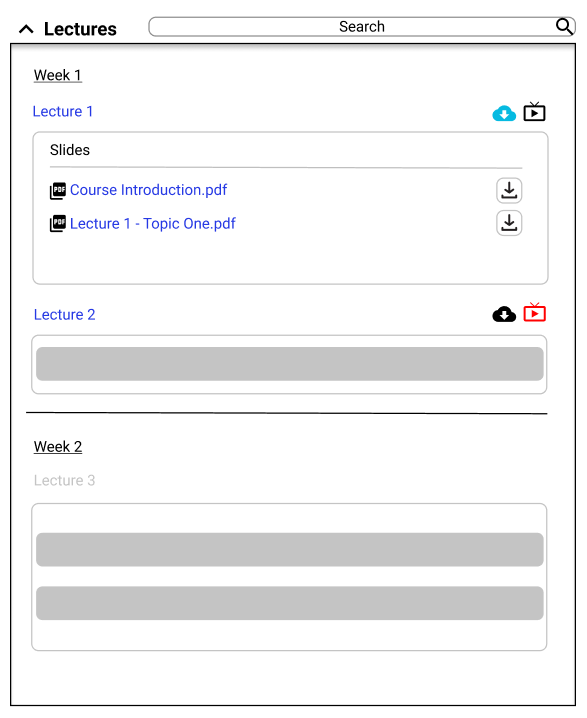
\includegraphics[scale=0.6]{lecture-main}
    \caption{Lecture User Interface}
\end{figure}

There will be an icon or text that will allow users to determine if it is live or completed. Students will be able to click on the relevant lecture row to view the 
content live or recorded. Additionally, there will be a feature to allow the lecture to be moved on the LMS screen (Video Pop Out). This feature will support users 
multitasking while watching their lecture videos. Course academics can click this row to start the relevant lecture and stream their classes. 

The user interface for lecture video streaming e will take inspiration from Canvas and will include white-boarding tools, a live chat, and a private messaging feature. There will be 
options to hide these tools and features to assist in user experience and accessibility. The lecturer will also be able to mirror their screen in the lecture. Also, the 
videos will also offer subtitles to assist users who have hearing impairments. 

\begin{figure}[h!]
  \centering
  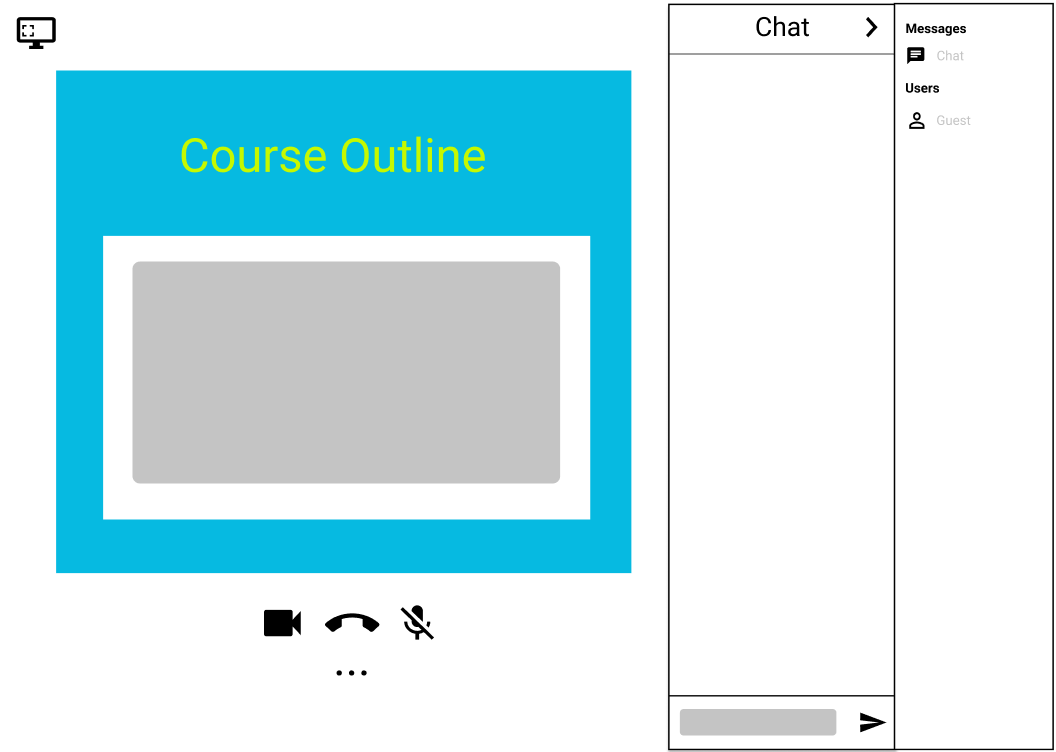
\includegraphics[scale=0.4]{video-stream}
  \caption{Video Streaming Features}
\end{figure}

\newpage
The tutorial video streaming design will be similar to the proposed design for the lecture videos. There will be the enabled addition of screen sharing between users present. 
This will be added to a toolbar during the tutorial session. The tutor will be able to check off attendance with a feature that automatically marks students 
off at an adjustable timeframe. For instance, the tutor may wish to consider attendance as 15 minutes in the tutorial class. 

\begin{figure}[h!]
    \centering
    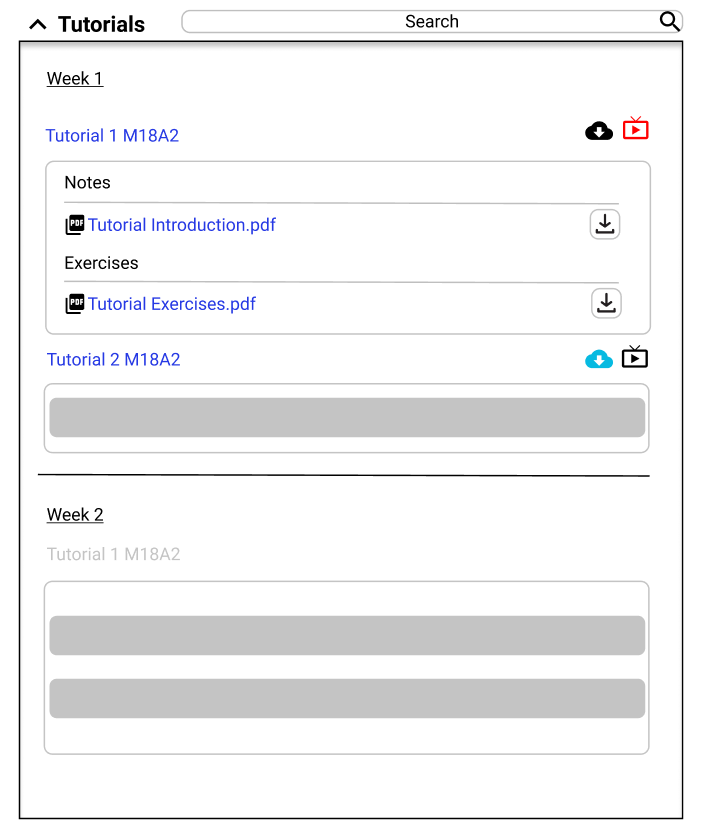
\includegraphics[scale=0.4]{tutorial-main}
    \caption{Tutorial User Interface}
\end{figure}
\newpage


\subsection{Functional Requirements}

\textbf{Lectures and Tutorials}
    \begin{enumerate}
    \item Users can toggle lectures and tutorials subsection visibility
    \end{enumerate}

\textbf{Video Streaming}
    \begin{enumerate}
    \item Users can watch a live lecture
    \item Users can watch a live tutorial
    \item Instructors can stream a live lecture
    \item Instructors can stream a live tutorial
    \end{enumerate}

\textbf{File System}
    \begin{enumerate}
    \item Users can search for a file
    \item Instructors can upload files to tutorials subsection
    \item Instructors can upload files to lectures subsection
    \item Users can download a recorded lecture
    \item Users can download a recorded tutorial
    \item Users can download tutorial files
    \item Users can download file files
    \item Users can view tutorial files
    \item Users can view lecture files
    \end{enumerate}

\subsection{Non-Functional Requirements}
  \begin{enumerate}
    \item Usability - The feature must be efficient and effective
    \item Performance - The feature must operate within a reasonable timeframe
    \item Aesthetics - The feature must be visually pleasing
    \item Learnabilty - The feature must be easy to learn and use
    \item Accessibility - The feature must accomodate varying users
    \end{enumerate}

\subsection{Timeline}
The timeline of the lecture and tutorials feature will depict the completion dates of each task for Thesis B and C.

\begin{figure}[h!]
    \centering
    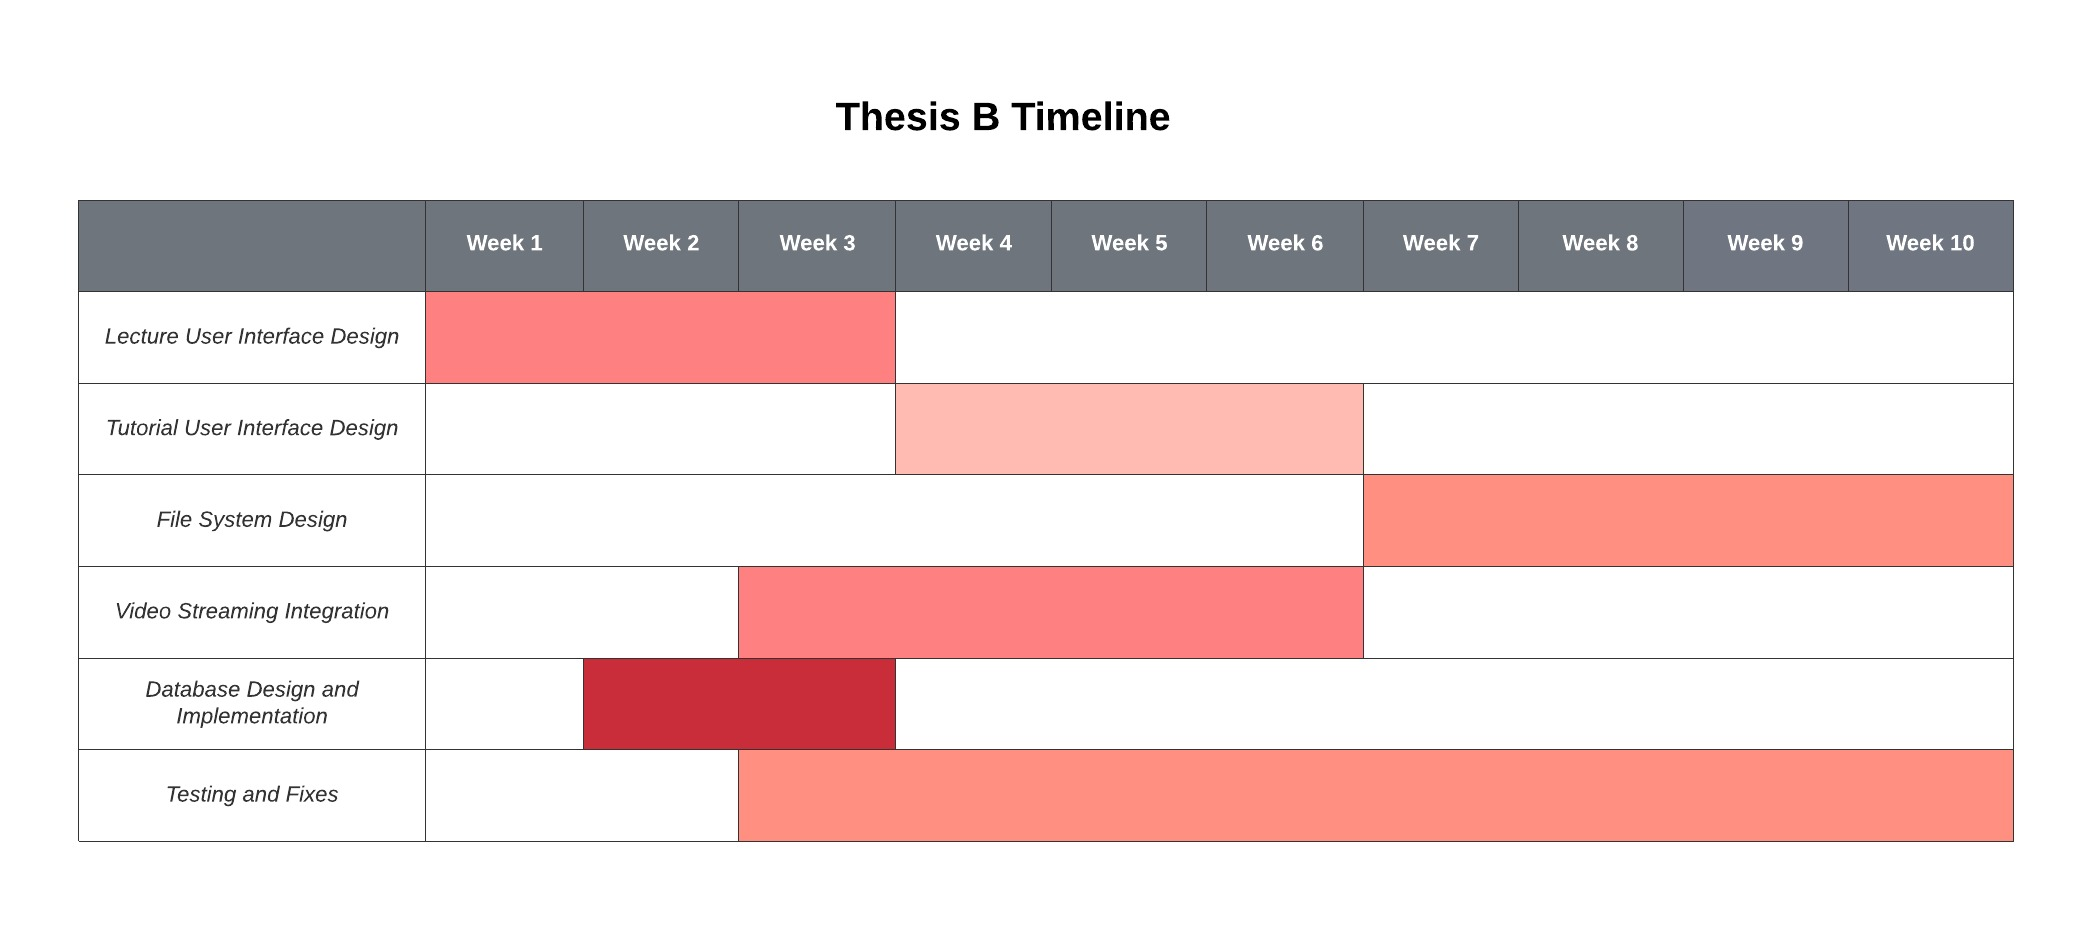
\includegraphics[scale=0.4]{lecturesTutorials_thesisB_gantt}
    \caption{Thesis B Timeline}
\end{figure}

For Thesis B the priority will be to finish the implementation for the lecture and tutorial interfaces in order to permit 
the implementation of the file system and video streaming features.

The video streaming and file system integrations will be implemented later in the term as these features are dependent on 
the lecture and tutorial user interfaces. Additionally, the video streaming feature will involve a third-party integration 
of a video streaming service into each lecture and tutorial sections. The file system feature will be implemented after the 
video streaming and lecture and tutorial interfaces as this is the final feature to create the MVP. The database design and 
implementation will be completed to store lecture and tutorial files. Moreover, a majority of the term will be spent on testing 
and fixes to any implemented features to ensure the success of implementation and designs.

\begin{figure}[h!]
    \centering
    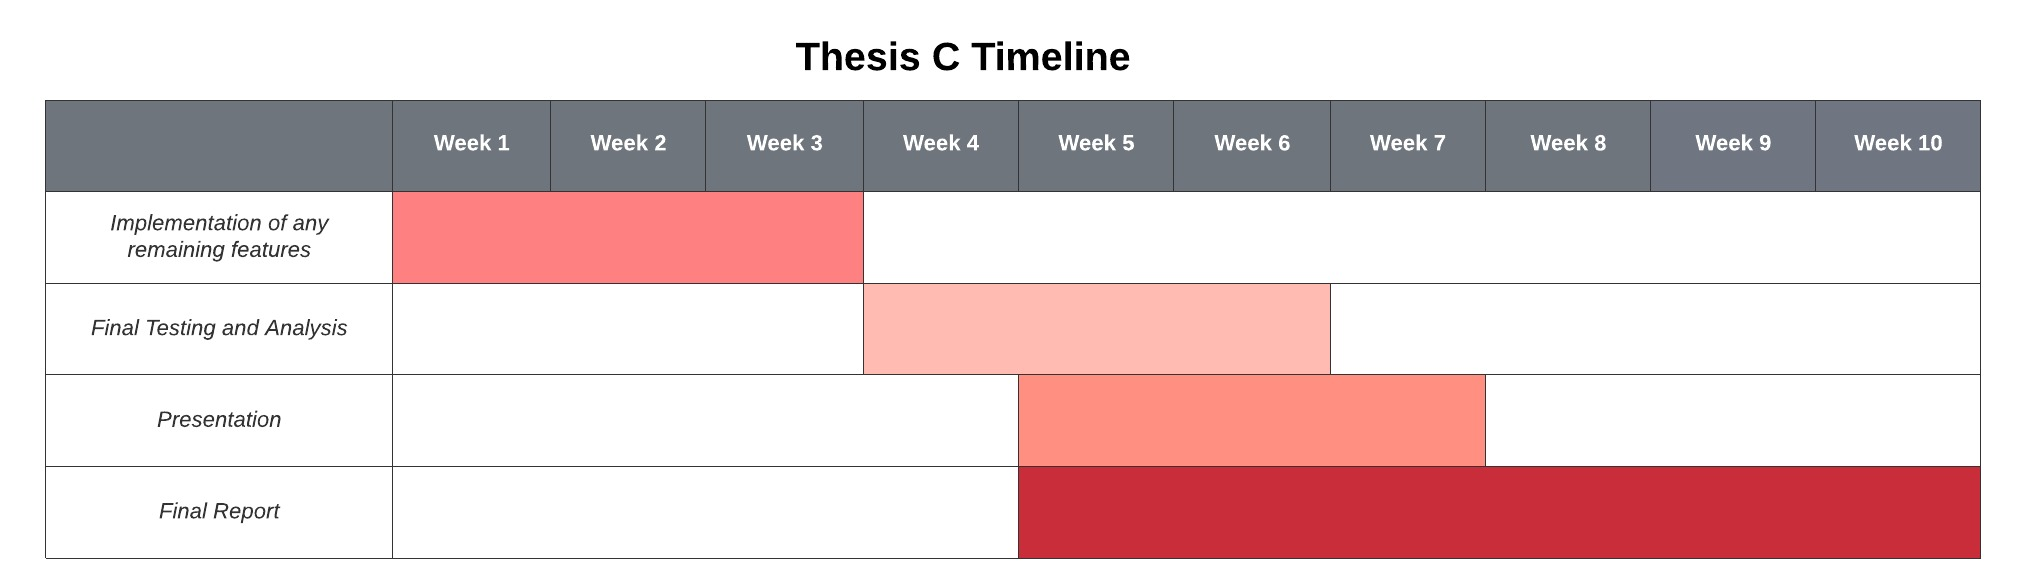
\includegraphics[scale=0.4]{lecturesTutorials_thesisC_gantt}
    \caption{Thesis C Timeline}
\end{figure}

In the Thesis C timeline, the implementation of any remaining features is prioritised to assure the lectures and 
tutorials features is complete. The next priority is the final testing and analysis of the completed feature to 
ensure the feature successfully satisfies the requirements. 

The remainder of the term will be utilised to work on the final demo presentation and the report. 

\subsection{Milestones}
The major milestones for the lecture and tutorials featured are outlined below:

\begin{enumerate}
\item Week 1 Term 2 2021 – Developing lecture user interface and database schema for storing lectures
\item Week 4 Term 2 2021 – Developing tutorial user interface and database schema for storing tutorials
\item Week 7 Term 2 2021 – Designing the file system, adding a file search system, and developing a database schema for tutorial and lecture file uploads
\item Week 9 Term 2 2021 – Integrating video streaming into lectures and tutorials sections
\item Week 5 Term 3 2021 – Final testing and fixes of the lecture and tutorials feature
\end{enumerate}

\subsection{Evaluating Results}
There will be an evaluation criterion which will be used to determine the success of the lectures and tutorials features in satisfying requirements and purpose.

\begin{enumerate}
    \item Aesthetics: Is the feature visually pleasing to the user
    \item Accessibility: Does the feature accommodate users with varying backgrounds (disabilities, children, etc)
    \item Performance: Does the feature run within a reasonable timeframe
    \item Usability/Learnability: Are the feature easy to learn and use
\end{enumerate}